\documentclass[10pt]{beamer}
\usepackage[spanish]{babel}
\usepackage[utf8]{inputenc}
\usepackage{color}
\usepackage{framed}
\usepackage{endnotes}
\usepackage{graphicx}
\usepackage{multicol}

\usetheme{Hannover}

\title{Exokernel}
\subtitle{An Operating System Architecture for \\  Application-Level Resource Managment}

\author{E. Mancuso\\ A. Mataloni\\ M. Miguel }

\date{16 de Junio de 2011}

\begin{document}
%-----slide------------------init--------------------
 \begin{frame}
  \titlepage
 \end{frame}
 \begin{frame}
  \tableofcontents
 \end{frame}
%----------------------------------------------------
\section{Introducción}
\subsection{Kernel Monolítico}
%-----slide------------------intro-------------------
\begin{frame}{Introducción}
La mayoría de los SO actuales utilizan kernels monolíticos, esto implica

\begin{itemize}
  \item Interfases de hardware genéricas
  \item Poca flexibilidad para la gran cantidad de aplicaciones existentes
  \item Implementaciones Ad-Hoc de abstracciones (Procesos, IPC, Archivos, etc)
  \item Ocultar informacion del Hardware a la aplicación
  \item Frena la innovacion en la implementación de abstracciones
\end{itemize}
\end{frame}

\subsection{Exokernel}
\begin{frame}

Es muy dificil implementar una abstracción que de un excelente rendimiento para toda aplicación existente y por ser desarrollada.\\[1em]

Por eso el exokernel propone cambiar la arquitectura monolítica por la siguiente \\[1em]

\begin{itemize}
  \item \textbf{Exokernel}: multiplexa los servicios de hardware de manera segura
  \item Primitivas de muy bajo nivel
  \item \textbf{Biblioteca SO}: Implementacion de abstracciones de alto nivel
\end{itemize}
\end{frame}

\subsection{Arquitectura}
\begin{frame}
\begin{figure}[H]
\centering
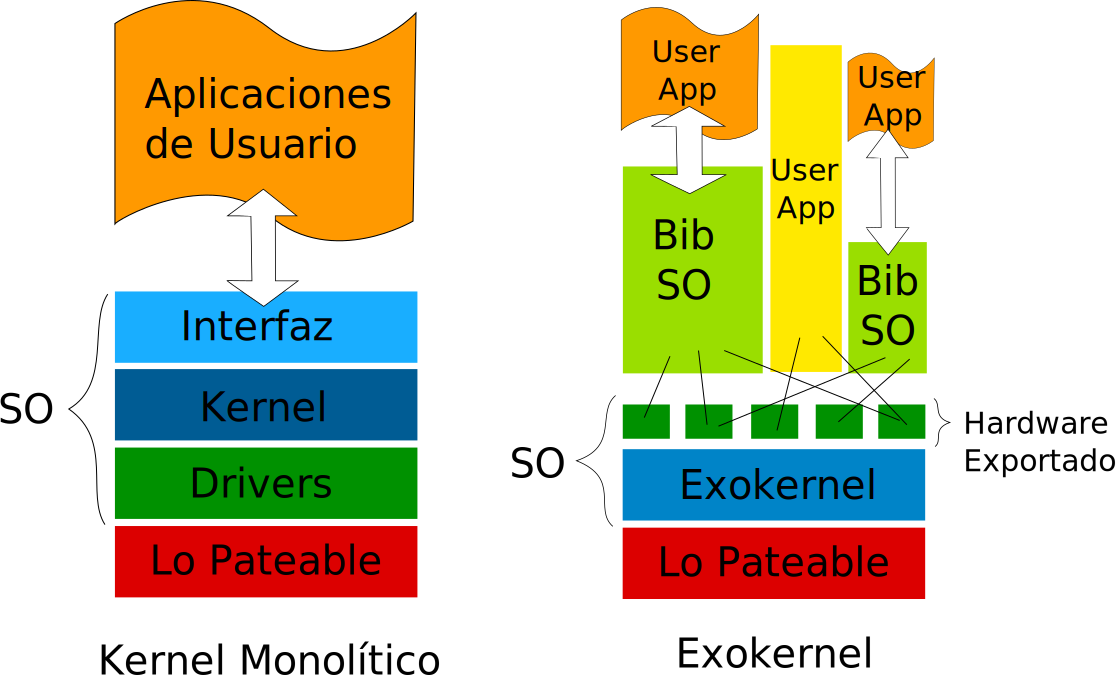
\includegraphics[scale=0.3]{grafico-kernel-exokernel.pdf}
\caption{Gráfico comparativo de los módulos en un kernel monolítico y un exokernel}
\end{figure}
\end{frame}

\subsection{Ventajas}
\begin{frame}
\begin{itemize}
  \item Interfaces más específicas
  \item Exportar el Hardware al usuario (programador de aplicaciones)
  \item La interfaz se define en el espacio de usuario.
  \item Controlar recursos desde nivel de usuario.
  \item Las aplicaciones conocen mejor que el SO qué recursos necesitan
\end{itemize}
\end{frame}

\section{Diseño}
\begin{frame}{Diseño}
Un \textbf{exokernel} se encarga de tres importantes tareas

\begin{itemize}
  \item Seguimiento de la asignación de recursos
  \item Garantizar la protección del uso de recursos o \textit{binding points}.
  \item Revocar el acceso a los recursos
\end{itemize}

\end{frame}


\subsection{Técnicas}
\begin{frame}
Para lograr implementar esta arquitectura hay que conocer las tres técnicas que utiliza el \textbf{exokernel} 

\begin{itemize}
  \item Secure bindings
  \item Visible resource revocation
  \item Abort protocol
\end{itemize}
\end{frame}


\subsubsection{Secure bindings}

\begin{frame}
\textbf{Secure bindings} \\[2em]

Es un mecanismo de protección que desacopla autorización del uso real de un recurso.\\[1em]

Las bibliotecas de Sistema Operativo pueden unirse o \textit{'bindiarse'} al Hardware para tener un mayor control sobre los eventos. \\[1em]  
La autorización se realiza sólo en el \textit{binding time}, esto permite separar la administración de la protección.\\[1em]

El \textbf{exokernel} interviene en todos los accesos a recurso.
\end{frame}

\subsection{Visible resource revocation}

\begin{frame}
\textbf{Visible resource revocation} \\[2em]

Permite a las \textbf{bibliotecas de sistema operativo} participar en el protocolo de revocación de recursos.\\[1em]

MARTIN: No se bien como explicarlo

\end{frame}


\subsection{Abort protocol}

\begin{frame}
\textbf{Abort protocol} \\[2em]

Es un protocolo para romper, a la fuerza, \textit{secure bindings} con las \textbf{bibliotecas de sistema operativo} que no cooperan o fallan al responder una solicitud de revocación.\\[1em]

El \textbf{exokernel} utiliza rompe todos los \textit{secure bindings} existentes con el recurso e informa a la \textbf{biblioteca de sistema operativo}. Ésta acción es registrada en un \textit{vector de recuperación} y la biblioteca recibe una excepción de \textbf{recuperación} para actualizar a quienes utilizan el recurso.
\end{frame}


\section{Experimentos}

\begin{frame}{Experimentos}
Para ver que esto efectivamente puede suceder, se implemento \textbf{Aegis} un exokernel y \textbf{ExOS}, una biblioteca de sistema operativo que implementa las abstracciones más importantes de los sistemas operativos. 

Los experimentos prueban estas hipótesis

\begin{itemize}
  \item Los \textbf{Exokernels} pueden ser muy eficientes
  \item La multiplexación segura de hardware se puede implementar de manera eficiente a bajo nivel.
  \item Las abstracciones de SO tradicionales se pueden implementar eficientemente a nivel de aplicación.
  \item Las aplicaciones pueden crear implementaciones de estas abstracciones con propósito específico.
\end{itemize}
\end{frame}

\begin{frame}
Aca tendriamos que poner las pruebas y esas cosas.... quizas algunos ejemplos 
\end{frame}

\section{Conclusión}

\begin{frame}{Conclusión}
 La conclusión que esat al final del paper, es justo la respuesta a cada hipotesis
\end{frame}



%----------------------------------------------------
\end{document}